\documentclass{article}
\usepackage[utf8]{inputenc}
\usepackage[margin=1in]{geometry}
\usepackage{listings}
\usepackage{eurosym}
\usepackage{graphicx}
\usepackage{hyperref}
\hypersetup{
	hyperindex=true
}
\usepackage{listings-rust}
\usepackage[utf8]{inputenc}
\usepackage[english]{babel}
\setlength{\parindent}{4em}
\setlength{\parskip}{1em}
\renewcommand{\baselinestretch}{1.5}
\usepackage{tikz}
\graphicspath{ {img/} }
\usepackage{listings}
\usepackage{float}
\usepackage[backend=bibtex,style=numeric,citestyle=numeric,sorting=none]{biblatex}
\addbibresource{bibliography.bib}
\author{Student Number: 170027195}
\title{DynoSesh: Dynamic Session Types}
\begin{document}
	\maketitle
	\pagebreak
	\tableofcontents
	\pagebreak
	\listoffigures
	\lstlistoflistings
	\pagebreak
	\section{Literature Review}
	\subsection{Session Types} \label{session types}
	When systems attempt to communicate over a protocol, the constraints of “acceptable” communication must be defined before and during transmission. The rubric to guarantee that protocol communication has fit within these boundaries, is however, less clear. If errors in transmission are to occur, future communication may become infeasible, and at worst, security issues could be introduced.
	
	Honda derived session types\cite{honda1993types, takeuchi1994interaction, honda1998language} as a strategy to mitigate potential issues that stem from the inability to properly check that an implementation of the protocol correctly matches the standard. In the 1994 paper\cite{takeuchi1994interaction} the need for an ``abstraction methodology'' to describe interactions between ``multiple, possibly distributed, parallel	processes'' is outlined, going on to state ``Such organization in turn may well be based on a type discipline, which ensures well-typed programs to behave in a principled fashion''. At its core, the session types proposal is for a language or method of describing the expected protocol communication, with a mechanism to check protocol implementations against the type definition, ensuring their correctness. 	Session types take influence from $\pi$-calculus\cite{milner1999communicating}, a process calculus used to model concurrent systems, with the 1994 paper\cite{takeuchi1994interaction} showing the authors adaption of $\pi$-calculus model of ``synchronous communication of values''.
	
	After a usable protocol representation has been outlined, often using the Scribble formal description language\cite{honda2011scribbling}, a checking process can occur to ensure that the implementation of the protocol matches its structure. The checking process can occur using one of three mechanisms, either statically, where the validity of the implementation is checked at compile time, dynamically at run time, or a hybrid approach, a combination of compile time assurance with a layer of run time checking is employed. Such a hybrid approach is described in Hu and Roshida, 2016\cite{hu2016hybrid} during which a static checker is used to validate the ``behavioural'' aspects of the system, generating finite state machines and restricting the operations that can be performed to those which adhere to one of the defined states. They then describe a ``light'' dynamically checked solution to ensure that defined channels of communication are used, and then are not re-used at a later date without the error in doing so violating the protocol definition.
	
	Modern research on session types considers ``multiparty'' systems, while early research largely considered a protocol implementation that exhibited communications between two parties, multiparty communication can have any numbers of participants in protocol communication. A 2008 paper by Honda et al.\cite{honda2008multiparty} gives an example of protocol communication which is extremely difficult to represent in a binary session, giving need for a solution which considers multiparty  communication. The consideration is for a system in which users can purchase expensive books from a seller, two buyers wish to purchase a single book together, the first buyer sends a book title to the seller, who responds to both the first and second buyer with the quote for the price of the book, the first buyer then communicates to the second buyer how much of the price they will pay, the second buyer then finally accepts the quote if they wish to proceed. The authors describe this as ``extremely awkward (if logically possible) to decompose this scenario into three binary sessions'' and express the need for the ability to express this as a single session, validated against a protocol implementation. The paper provides an expansion of the initial session types language found in\cite{takeuchi1994interaction, honda1998language} which incorporates the ability to consider protocols which express the communication between multiple parties over a protocol.
	\subsubsection{Static Session Type Implementations}
	Static implementations of session types, as expressed in section \ref{session types} perform the checking of the validity of the protocol implementation at compile time. There are multiple real world implementations for a host of languages that implement such a system in varying forms, from Java through to Haskell\cite{lindley2016embedding}. 
	
	Some statically typed implementations, such as SessionJ\cite{hu2008session} for Java, implement extensions to the language they are built for to provide this functionality. SessionJ implements a \texttt{protocol} keyword and subsequent domain specific language for expressing the contents of a protocol specification, an example of this is show in listing \ref{lst:sessionJ}. The communication of the structure of a protocol may not be possible, or elegant, without creating such an extension, in the Hu et al. paper\cite{hu2008session} an integration of the language extension into the wider Java compilation process is implemented. They describe three layers of compilation and execution, with the first layer being the "SessionJ source code", the Java code with the protocol extensions implemented, this then is translated into Java by the SessionJ compiler, before running on the JVM with SessionJ run time libraries to ensure that the sending an receiving of messages over the protocol is implemented correctly.
	\begin{lstlisting}[language=java, frame=single, numbers=left, caption=An implementation of a protocol to place an order by Hu et al. to showcase the capabilities of SessionJ\cite{hu2008session}, label={lst:sessionJ}]
protocol placeOrder {
	begin. // Commence session.
	![ 	// Can iterate:
		!<String>. 	// send String
		?(Double) 	// receive Double
	]*.
	!{ 	// Select one of:
		ACCEPT: !<Address>.?(Date),
		REJECT:
	}
}

	\end{lstlisting}
	Other approaches to the implementation of statically checked session types within a language do not extend or modify the language to achieve this functionality. One example, for the Rust programming language\cite{jespersen2015session} uses chained type parameters to achieve their goal, they provide an example of the implementation of an ATM shown in listing \ref{lst:rustlang}, which can take withdrawals and deposits. This displays the syntax with which the session type framework is implemented, through the chaining of a number of calls to types, with \texttt{Recv<>} being to receive a value, and \texttt{Send<>} to send a value over the protocol. Any larger implementation that the ATM example would begin to have extremely long and convoluted type definitions to express the structure of the protocol, effectively becoming a domain specific language for the expression of a protocol's operation within another language. Due to these complexities, such an approach, particularly in the case of statically checked session types which has some form of compilation step to check the validity of the implementation at compile time, does not seem to be favoured.
\begin{lstlisting}[language=rust, frame=single, numbers=left, caption=An implementation of an ATM using session types in Rust\cite{jespersen2015session}, label={lst:rustlang}]
	type Atm = Recv<Id, Choose<Rec<AtmInner>,Eps>>;
	type AtmInner = Offer<AtmDeposit, Offer<AtmWithdraw, Quit>>>;
where:
	type Id = String;
	type Quit = Eps;
	type AtmDeposit = Recv<u64, Send<u64,Var<Z>>>;
	type AtmWithdraw = Recv<u64, Choose<Var<Z>,Var<Z>>>;
	\end{lstlisting}
	\subsubsection{Dynamic Session Type Implementations}
	There are also a wide number of dynamically checked session type implementations for a host of languages and technologies, one such tool is Session Python for the Python programming language\cite{neykova2013spy}. The Neykova et al. paper stresses the need for static implementations to extend the language they are built for, ``Static session type checking in these mainstream languages, however, requires support in the form of the language extensions and pre-compiler processing to be tractable''. The implementation instead uses Scribble\cite{honda2011scribbling} to express the structure of protocol communication, this protocol structure is then enforced at run time. 
	
	In comparison to statically checked session types, where the correctness of an implementation is proved at compile time, runtime checking of session types require some level of coordination between actors using session types to check the status of their protocol communication amongst each other. In a distributed context, the global protocol communication standard shared amongst actors must be disseminated to a local context per each actor and enforced at that level locally. Without this, a single actor would be aware of the success of protocol communication locally, but would have no knowledge of the success of protocol communication between other actors. The Session Python runtime provides each defined role in the protocol with its own local success parameters ``Scribble (i.e. syntactic) local protocol specifications for each participant (role) defined in the protocols''\cite{neykova2013spy}, this ensures that there is global compliance with the protocol, even when actors are only aware of the constraints on their local context.
	\subsection{The Actor Model}
	The actor model introduces a strategy for the control of parallel computation to avoid potential errors, such as deadlock or race conditions. The actor model places a number of rules upon what an actor can do, an actor has 3 valid “actions”; to create another actor, to send a message to another actor or to instruct itself on how to deal with the next message it receives.
	
	Each actor is assigned with some concept of an “address”, this provides a mechanism for an actor to communicate with other actors within the system, passing messages between each other as needed. When messages are passed from one actor to another, they are stored in the actors individual task queue; these tasks are then executed one by one, with an actor polling the queue for new tasks after a single unit of work has been completed. Actors also have some form of private state, this allows for an actor to be aware of information relating to the current status of its execution and the execution of tasks prior to the task is is currently executing. Through these three components, the address, the individual task queue and the private state, a sense of the decoupled nature of the actor model can be realised. The goal is to fully abstract and decouple actors from each other, with communication and synchronisation between actors only occurring via the message passing framework.
	
	There are a variety of implementations of the actor model, some research-focused languages are designed entirely entire around the concept, such as Rosette\cite{Tomlinson:1988:ROC:67387.67410}. Other implementations that are more popular amongst the wider general purpose programming community are Erlang’s concurrent and distributed computation utilities, and Akka\cite{akkawebsite}, which provides an actor model framework for languages that run on the Java Virtual Machine, such as Scala, Java and Kotlin. 
	Erlang is a functional programming language which has built in message passing capabilities for communication between processes. The \texttt{!} operator is used to send a message to the identified process, an example of a program which sends the word “Ping” to an actor, which then returns “Pong” a number of times is listed in the Erlang documentation\cite{ErlangConcDocs} as displayed in listing \ref{lst:erlangDocs}.
	\begin{lstlisting}[label={lst:erlangDocs}, language=erlang, frame=single, numbers=left, caption=Ping Pong in concurrent Erlang\cite{ErlangConcDocs}]
-module(tut15).

-export([start/0, ping/2, pong/0]).

ping(0, Pong_PID) ->
	Pong_PID ! finished,
	io:format(``ping finished~n'', []);

ping(N, Pong_PID) ->
	Pong_PID ! {ping, self()},
	receive
		pong ->
			io:format(``Ping received pong~n'', [])
	end,
	ping(N - 1, Pong_PID).

pong() ->
	receive
		finished ->
			io:format(``Pong finished~n'', []);
		{ping, Ping_PID} ->
			io:format(``Pong received ping~n'', []),
			Ping_PID ! pong,
			pong()
	end.

start() ->
	Pong_PID = spawn(tut15, pong, []),
	spawn(tut15, ping, [3, Pong_PID]).
	\end{lstlisting}
	Akka's implementation of the actor model provides a similar construct, actors exist within a wider network and pass messages to each other to execution methods. However, unlike Erlang, it provides this as library functionality on top of other general purpose programming languages that run on the Java Virtual Machine. Akka allows developers to create a tree hierarchy of actors, with individual actors organised into groups, as shown in figure \ref{fig:AkkaTree}. This hierarchy is used to enforce concurrency amongst and between groups, with actors inside a group running concurrently as well as the groups themselves. The hierarchical structure of the actor grouping also helps to isolate errors, if a failure of an actor occurs within a group, due to the isolated nature of the actor model this can be dealt with at the group level without requiring a full system-wide recovery process.
	\begin{figure}[H] \label{fig:AkkaTree}
	\caption{Akka actor structure example}
	\centering
	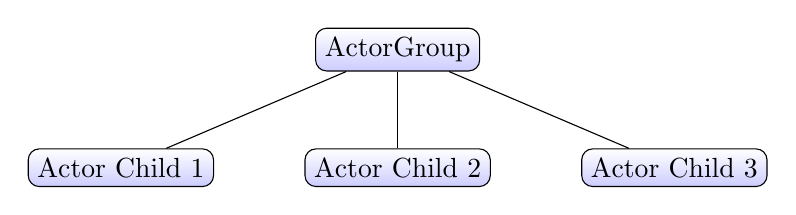
\begin{tikzpicture}[sibling distance=10em,
every node/.style = {shape=rectangle, rounded corners,
	draw, align=center,
	top color=white, bottom color=blue!20}]
\node {ActorGroup}
child { node {Actor Child 1} }
child { node {Actor Child 2} }
child { node {Actor Child 3} };
\end{tikzpicture}
	\end{figure}
	\subsection{Security Problems Regarding Protocols}
	There is a wide ranging literature on the security of protocols and their usage, covering strategies to guarantee secure communication and vulnerabilities that exist within current protocols. One such protocol is Kerberos\cite{neuman1994kerberos} which provides the ability for actors to communicate securely over an unsecured network. The protocol is complicated, with many encrypted messages sent back and forth from client to client to prove the identity of an actor to prevent impersonation. An unsound implementation of the protocol could mean that vulnerabilities exist within communications between clients that were assumed to be secure, exposing the users unwittingly to harmful actors.
	
	Faulty implementations of protocols have existed in the wild and potentially have left users of the implementation at risk of harm. Apple's implementation of the secure sockets layer\cite{elgamal1997secure} (SSL), protocol in iOS 6.0 was vulnerable to man in the middle attacks\cite{bland2014finding} which would allow for a hostile actor to ``eavesdrop'' on assumed secure communication between two parties. The code section which introduce the bug, shown in listing \ref{lst:vulnios} occurred when the second \texttt{goto fail;} command was automatically executed on every time the \texttt{update()} function returned true, jumping over a critical final section of the algorithm. Such a bug is hard to identify, even after code review, yet has a wide effect on the sense of trust that users have in their devices to facilitate secure communication, the importance on correct and secure implementations of protocols is paramount.
	\begin{lstlisting}[label={lst:vulnios}, language=c, frame=single, numbers=left, caption=The vulenarble code section in iOS 6.0's SSL implementation\cite{bland2014finding}]
if ((err = SSLHashSHA1.update(
	&hashCtx, &signedParams)) != 0)
	goto fail;
	goto fail;
	\end{lstlisting}
	\section{Implementation}
	\subsection{Domain Specific Language}
	Users having the ability to express the structure of complex protocols easily is key to the adoption of the library by a wider user-base. It is paramount that this is made as simple as it possibly can, to improve both usability when creating the protocol structure and comprehension when checking it at a later date. As expressed in the literature review, one such standard approach is the Scribble\cite{honda2011scribbling} domain description language, where users create protocols and then use tools to compile the contents to an implementation usable with their language of choice. In a library sense, however, this is imperfect, it requires an extra layer of knowledge from users outside of the normal language paradigm, it increases the learning curve, potentially putting off new users, and requires some form of parsers and compilation process which could prove difficult to implement in the time constraints of the project.
	
	Within the domain specific language discourse there is a distinction made between so called ``external'' and ``internal'' domain specific languages\cite{Fowler:2010:DSL:1809745}. External implementations, such as Scribble, are written in a language outside of the implementation language, often within a completely separate file, they are then parsed and comprehended by the runtime that has been implemented to execute them. Internal domain specific languages, however, are written within their implementation language, complying validly with the grammar. A valid expression written using an internal domain specific language will also be valid within the wider implementation language that was used to build it. Fowler provides two examples of this in his book, showing the difference between ``standard'' APIs, shown in listing \ref{lst:normalJavaAPI}, and an implementation of an internal domain specific language that utilises method chaining displayed in listing \ref{lst:intDSLJava}, both providing the same result.
	
	\begin{lstlisting}[label={lst:normalJavaAPI}, language=java, frame=single, numbers=left, caption=Object construction in a normal API\cite{Fowler:2010:DSL:1809745}]
Processor p = new Processor(2, 2500, Processor.Type.i386);
Disk d1 = new Disk(150, Disk.UNKNOWN_SPEED, null);
Disk d2 = new Disk(75, 7200, Disk.Interface.SATA);
return new Computer(p, d1, d2);

	\end{lstlisting}
	
\begin{lstlisting}[label={lst:intDSLJava}, language=java, frame=single, numbers=left, caption=Object construction in a method chained internal Domain Specific Language\cite{Fowler:2010:DSL:1809745}]
computer()
	.processor()
		.cores(2)
		.speed(2500)
		.i386()
	.disk()
		.size(150)
	.disk()
		.size(75)
		.speed(7200)
		.sata()
	.end();

	\end{lstlisting}
	While the latter of the two listings does not look like "regular" Java code, or follow normal recommended standards surrounding line length, it still compiles. If a wider scope than just the code samples relationship to normal Java code is taken however, the purpose of the exercise reveals itself. The internal DSL allows for the abstraction of expressing what the user wants away from normal object creation. Users can now think in terms of ``computers'' which have ``processors'' and ``disks'' and allow for the internal DSL's workings to create the object they need for them. This approach can be applied to the construction of graph representation of protocols, allowing for users to place the structure of the graph at the heart of their reasoning, separate from object construction.
	
	An example of the API DynoSesh exposes for constructing protocols is shown in listing \ref{lst:dynoSeshIntDSL}. This will result in a protocol of two nodes, with one start node that accepts a single \texttt{TestClass} sent over the protocol from actor 0, and then another node which will recursively accept more \texttt{TestClass} objects from actor 0 infinitely. During the construction of a protocol, nodes that are declared earlier in the process need to be able to potentially access those which are defined later, therefore no connections between objects are instantiated until the \texttt{NodeBuilder.build()} method is called to create the protocol. There are a number of error checking procedures controlling protocol construction to ensure that invalid protocols cannot be produced, these include but are not limited to ensuring that a single protocol cannot have more than one start node.
	\begin{lstlisting}[label={lst:dynoSeshIntDSL}, language=java, frame=single, numbers=left, caption=Construction of a DynoSesh graph using the internal DSL]
ProtocolBuilder protocolBuilder = new ProtocolBuilder();
Protocol protocol = protocolBuilder
	.node()
		.payload(null)
		.connection()
			.actor(``0'')
			.to(``1'')
	.node()
	.payload(TestClass.class)
		.connection()
			.actor(``0'')
			.to(``1'')
	.build();
	\end{lstlisting}
	The internal DSL also allows for the creation of branches, with one node able to have multiple connections, there are a number of paths that communication can take throughout the protocol graph depending on what transmissions occur.
	\pagebreak
	\printbibliography
\end{document}